%
%	Begrifflichkeiten
%

\pagebreak
\section{TLS \& mTLS}

\onehalfspacing

\subsection{TLS}

TLS stands for Transport Layer Security.\footnote{See \textit{NIST (2011)}: Glossary. \cite{nistTLS}} It's a critical internet
security protocol that encrypts the connection between a user's computer
and their website or service. TLS scrambles the data sent between the
computer and the service, turning it into an unreadable code. This
prevents hackers from intercepting and stealing information (passwords,
credit card details, personal data, etc.). TLS also verifies that the
service is legitimate and not a fake one trying to steal information; it
ensures that the data sent between computers and services has not been
tampered with or altered during transmission.\footnote{See \textit{Internet Society (2025)}: TLS Basics. \cite{tlsBasics}}

TLS is the foundation of secure online communication. Without it, data
would be vulnerable to interception and theft. TLS helps keep online
activity private, preventing eavesdropping and unauthorized access to
information. TLS certificates, or SSL certificates, are a sign of
confidence. Websites with TLS encryption display a padlock icon in the
browser, reassuring users that their connection is secure.

TLS uses a combination of symmetric and asymmetric
cryptography. Symmetric cryptography encrypts the data, while
asymmetric cryptography authenticates the server and exchanges the
symmetric encryption key.\footnote{See \textit{ENTRUST (2025)}: What is TLS. \cite{whatIsTls}}

TLS is an essential part of internet security. It helps to
protect sensitive information from being intercepted and stolen. SSL was
the predecessor to TLS, which is more modern and secure. While the terms
are sometimes interchangeable, TLS is the more modern protocol.

TLS is essential for protecting privacy and security online. Its
technology allows for secure online transactions, browsing, and
communication.

\subsection{mTLS}

Mutual TLS (mTLS) is a type of authentication that requires both the
client and the server to authenticate each other. This contrasts with
traditional TLS, which only requires the server to authenticate itself
to the client.\footnote{See \textit{Google Cloud (2025)}: Mutual TLS overview. \cite{mutualTls}}

mTLS provides additional protection by ensuring that the client and the
server are who they claim to be. This can help prevent man-in-the-middle
attacks and other security threats. mTLS can authenticate users and
devices, which can be helpful in various situations, such as accessing
sensitive data or applications. mTLS can also help protect the
confidentiality of user data by ensuring that only authorized parties
can access it.

mTLS is very important in securing APIs by ensuring only authorized
clients can access them. It can also protect sensitive data, such as
financial or medical information, and authenticate users and devices
when they access sensitive resources.

mTLS is a valuable security tool for protecting sensitive data and
applications. It is beneficial when high levels of security and
authentication are required, such as when the NIS2 requirements need to
be met.

\subsection{Microservice Architecture}

Microservice architecture is a software development approach in which an
application is structured as a collection of small, autonomous services
modeled around a business domain. It can be compared to a bustling city
comprising specialized districts (aka services) that work together to
make the city function. Each district has its infrastructure, team, and
way of doing things, but they all contribute to the overall city
experience.\footnote{See \textit{Google Cloud (2025)}: What Is Microservices Architecture. \cite{whatIsMS}}

Each microservice is designed to perform a specific business function in
a micro-service application. They are small enough to be developed,
deployed, and maintained independently. Microservices operate
independently. A failure in one service does not bring down the entire
application. Microservices can also be updated or deployed without
affecting other services.

They are decentralized, with no central database or monolithic code
base. Each microservice can choose the technology stack (programming
language, database, etc.) best suited for its specific task, allowing
for greater flexibility and innovation.

Microservices communicate with each other through well-defined APIs,
often using lightweight protocols like REST or message queues. This
loose coupling minimizes dependencies between services, making them more
independent. Microservices can be deployed and scaled independently. For
example, if one service is experiencing high traffic, it can be scaled
to increase its capacity without scaling the entire application.

Microservices are a good fit for large, complex applications. They can
break down complexity into smaller, manageable parts and application
parts that can scale independently. They are also well-suited for
applications with varying workloads.

Microservices generally follow an API-first design. They communicate
through well-defined APIs, which act as contracts between services and
ensure interoperability. A common choice is RESTful APIs using HTTP.

Microservices offer a powerful approach to building complex applications
but require careful planning and execution. Understanding the trade-offs
and challenges are crucial for successful implementation.

\subsection{Service Mesh}

A service mesh is an infrastructure layer between application services
and the underlying network. It is designed to make communication between
microservices easier, more reliable, and secure and has a dedicated
traffic management and security layer. It handles all the complexities
of inter-service communication, allowing the application code to focus
on business logic.\footnote{See \textit{Hamilton, C. (2024)}: What is a service mesh. \cite{whatIsMesh}}

A Service Mesh controls how traffic flows between services. This
includes routing, load balancing, retries, timeouts, and fault injection
(testing resilience). It can intelligently route requests based on
various criteria, such as versioning, A/B testing, or canary
deployments. It secures communication between services. This includes
mutual TLS (mTLS) authentication, authorization, and encryption, which
we will analyze later. With mTLS, it ensures that only authorized
services can communicate with each other and that all communication is
encrypted.

A Service Mesh also provides insights into the behavior of
microservices. This includes metrics, tracing, and logging. It allows
for monitoring the health and performance of all services in the mesh
and quickly identifying any issues.

A service mesh typically uses a ``sidecar'' proxy pattern. This means a
small proxy (the sidecar) is deployed alongside each microservice
instance in the container. All traffic to and from the microservice
flows through this sidecar proxy, which is managed by a control plane
configuring the mesh and collecting telemetry data.

A service mesh is a powerful tool for managing and securing
communication between microservices. It can simplify development,
improve security and resilience, and enhance observability. However, it
also adds complexity to the application landscape, so it's essential to
carefully consider the trade-offs before implementing one.

\subsection{Benefits of a Service Mesh}

Microservices often need to communicate with each other, which can
involve intricate tasks like service discovery, load balancing, and
handling network issues. A service mesh abstracts these complexities
away, allowing developers to focus on the core logic of their
microservices. It provides a uniform way for services to communicate,
regardless of the language or framework in which they are written. This
ensures consistency and simplifies development.

A service mesh can enforce mTLS, encrypting communication between
services and verifying the identity of both the client and the server.
This significantly strengthens security and prevents unauthorized
access. It also allows for defining and enforcing security policies
across the entire microservices ecosystem from a central point,
simplifying security management.

A service mesh provides detailed insights into the behavior of the
microservices, including metrics, tracing, and logging. This makes it
easier to monitor their health and performance and identify issues.

Service meshes offer features like circuit breaking, retries, and
timeouts, which make microservices more resilient to failures. This
helps prevent cascading failures and ensures your application remains
available even when some services are down.

Thus, a service mesh acts as a dedicated infrastructure layer for the
microservices landscape, handling the complexities of inter-service
communication, security, observability, and resilience. This allows
developers to focus on building great applications while operations
teams can effectively manage and monitor the microservices ecosystem.

\subsection{Benefits of mTLS}

Microservices often communicate over a network, making them vulnerable
to interception and eavesdropping. mTLS enforces a ``zero trust'' model,
where every service must authenticate itself regardless of its location
within the network. This is critical in a microservice environment where
services might be deployed across different environments or clouds.\footnote{See \textit{Patil, K. (2023)}: Why Mutual TLS is critical. \cite{whyCritical}}

mTLS verifies the digital certificates of the client and server to
ensure that they are who they claim to be. This prevents unauthorized
services from impersonating legitimate ones, a key concern in a
distributed microservice system. mTLS also encrypts all communication
between services, protecting sensitive data from being intercepted and
read. This is paramount in microservices, as data might travel through
various network segments.

mTLS establishes a straightforward and automated way for services to
trust each other. No complex key management or manual configuration is
needed for each service interaction. The service mesh (or other
infrastructure) handles certificate distribution and validation. Each
service will have a verifiable identity. This simplifies auditing,
logging, and access control.

mTLS makes Man-in-the-Middle attacks significantly harder. To intercept
communication, an attacker would need to possess the private key of a
legitimate service. Also, because each service is authenticated, it's
much more challenging for a malicious service to ``spoof'' or impersonate a
legitimate one.

Many industries have strict data security and privacy regulations. mTLS
can help organizations meet these requirements by providing strong
authentication and encryption of inter-service communication. This is
increasingly important as microservices handle increasingly sensitive
data.

Microservices' distributed nature increases their attack surface and
mTLS helps secure the many communication points between services.
Microservices are often deployed and scaled dynamically, and mTLS
provides an automated way to handle security in this fluid
environments. Microservices rely heavily on each other. If one service
is compromised, it can potentially expose others, and mTLS limits a
compromised service's ``blast radius'' by ensuring that communication
with other services is always secured.

mTLS is a fundamental security practice for microservice architectures.
It provides strong authentication and encryption and simplifies security
management, making it an essential tool for protecting sensitive data
and ensuring the integrity of inter-service communication. When
integrated with a service mesh, mTLS becomes even more powerful and
easier to manage.

\subsection{Linkerd}

Linkerd is a lightweight and straightforward service mesh designed for
Kubernetes. It manages and secures communication between microservices,
providing a dedicated traffic management and security layer without the
complexity associated with service meshes.\footnote{See \textit{Linkerd (2025)}: Why Linkerd. \cite{linkerD}}

Linkerd's minimalist design focuses on providing essential service
mesh functionalities without unnecessary complexity. This makes
installing, configuring, and operating easier than other service meshes.
Linkerd is known for its straightforward installation process and
user-friendly CLI.

Linkerd uses a purpose-built, ultra-lightweight proxy written in Rust
and is designed to have a minimal performance impact on the
applications. It aims to be as efficient as possible, adding little
overhead to service communication.

Linkerd enables mTLS by default, which encrypts communication between
services and ensures that only authorized services can communicate. It
promotes a zero-trust security model in which every service must
authenticate itself regardless of its location within the network.\footnote{See \textit{Morgan, W. (2024)}: Zero trust network security in Kubernetes. \cite{zeroTrust}}

Linkerd is a service mesh focusing on simplicity, performance, and
security. It's a good option for teams that want a lightweight and
easy-to-use service mesh for their Kubernetes deployments.

\subsection{Istio}

Istio is a popular, open-source service mesh that sits atop a container
orchestration platform like Kubernetes. It helps connect, secure,
control, and observe microservices; it is a smart infrastructure layer
that manages communication between services.\footnote{See \textit{Google Cloud (2025)}: What Is Istio. \cite{whatIsIstio}}

Istio offers fine-grained control over traffic flow between your
microservices. This includes Routing, Load Balancing, Fault Injection,
and Traffic Splitting.

Istio provides robust security features, such as Mutual TLS (mTLS),
Authorization and Authentication. Istio also allows you to define and
enforce policies across all microservices, such as Rate Limiting and
Quota Management.\footnote{See \textit{Istio (2025)}: Security. \cite{istioSecurity}}

Istio uses a ``sidecar'' proxy pattern. A lightweight proxy (typically
Envoy) is deployed alongside each microservice instance. All traffic to
and from the microservice flows through this sidecar proxy. Istio's
control plane manages these sidecar proxies, configuring them with the
desired traffic management, security, and policy rules.

Key Components of Istio:

\begin{itemize}
	\item Pilot: The primary component for traffic management. It configures the Envoy proxies based on the traffic rules you define
	\item Citadel: Handles security, including certificate management for mTLS
	\item Galley: Manages Istio's configuration.
\end{itemize}

Istio is most beneficial for complex microservices architectures and
applications that require high levels of security and resilience.

Istio is a powerful and feature-rich service mesh that can significantly
simplify the management and security of microservices. However, it also
adds complexity to your infrastructure, so it's important to consider
whether it's the right solution.


\subsection{Rancher}

To easily manage the service mesh installation on a Kubernetes cluster, we can turn to SUSE Rancher.

What is Rancher? The Rancher Labs website states it is "[...] a complete software stack for teams adopting containers. It addresses the operational and security challenges of managing multiple Kubernetes clusters while providing DevOps teams with integrated tools for running containerized workloads."\footnote{\textit{Rancher Labs (2025)}: Enterprise Kubernetes Management. \cite{rancher}}

Using a user-friendly GUI, Rancher provides a management platform for centrally managing multiple Kubernetes clusters in Enterprise IT. It also offers application development integration tools and robust enterprise-grade security and governance features. For operations, Rancher provides integrated solutions for logging, monitoring, and auditing, as well as many other features, such as CIS scans or a built-in service mesh.

The classic Rancher GUI looks like this:

\begin{figure}[H]
\centering
\caption {Rancher Dashboard}
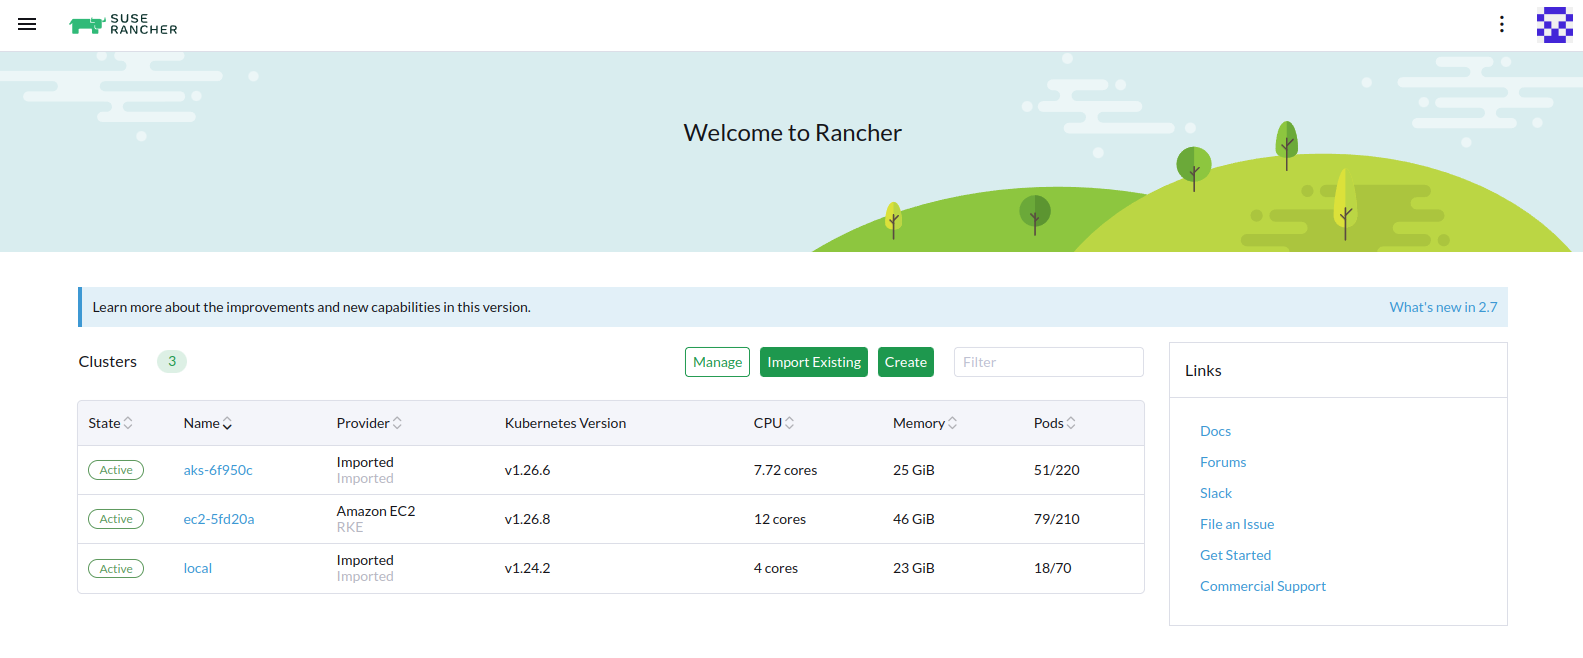
\includegraphics[width=\linewidth]{images/rancher-dashboard.png}
\label{fig:rancherDashboard}
\end{figure}
